\documentclass[../main.tex]{subfiles}
\begin{document}
\setchapterimage[6.5cm]{Images/intro.jpg}
\setchapterpreamble[u]{\margintoc}
\chapter[Introduction]{Introduction\footnotemark[0]}
\labch{intro}
\section{Dimensional Analysis and Energy Scales}
We start our discussion about the Standard Model by introducing some fundamental concepts about dimensional analysis. For our purposes, we work with \textbf{natural units}, i.e. $\hbar=c=1$. It follows that:
\begin{itemize}
    \item $[m]=[E]$ since $E=mc^2$ 
    \item $[t]=[E^{-1}]$ since $\Delta E\Delta t\gtrsim\hbar$
    \item $p^\mu=(E,\Vec{p})$ and we have that $[x]=[E^{-1}]$
    \item the Lagrangian density $\pazocal{L}$ has dimension $[\pazocal{L}]=[E^4]$ because it has to be $[S]=\left[\int d^4x\pazocal{L}\right]=0$
    \item The fields we work with have dimensions:
    \[
    [\phi]=[E] \quad [\partial_\mu\phi]=[E] \quad [\Psi]=[E^{3/2}] \quad [A_\mu]=[E]
    \]
\end{itemize}
For the couplings, we observe that $e\overline{\Psi}\gamma^\mu A_\mu\Psi$ must have dimension $E^4$ therefore it has to be $[e]=[E^0]$. The same reasoning applies for $G_{\text{F}}\overline{\Psi}\Psi\overline{\Psi}\Psi$ and we obtain $[G_{\text{F}}]=[E^{-2}]$.

The typical energy scale we are going to use is GeV, while the masses we are interested in are:
\[
\left\{
\begin{aligned}
&\text{Leptons: } &&m_e=0.511\text{ MeV} &&m_\mu=105\text{ MeV}  &&m_\tau=1.77\text{ GeV}\\
&\text{Light quarks: } &&m_u=2.5\text{ MeV}  &&m_d=5.0\text{ MeV}  &&m_s=0.105\text{ GeV}\\
&\text{Heavy quarks: } &&m_c=1.27\text{ GeV}  &&m_b=4.20\text{ GeV}  &&m_t=173\text{ GeV}
\end{aligned}
\right.
%Grazie a Giorgio che mi ha fatto allineare tutto per bene (giovedì 20 ottobre 2022, nell'Ufficio)
\]
In quantum chromodynamics (QCD) the scale is given by the quantity $\Lambda_{\text{QCD}}$. Its value is $\Lambda_{\text{QCD}}=332\pm17$ MeV when the energy involved in the process allows only to produce the light quarks, i.e., energies below 1.27 GeV. At higher energy, $\Lambda_{\text{QCD}}=210\pm14$ MeV, above the bottom quark mass. This gives mass to elementary fields:
\[
\left\{
\begin{aligned}
&m_p=938\text{ MeV}=g_p\Lambda_{\text{QCD}} \quad m_n=939\text{ MeV}=g_n\Lambda_{\text{QCD}}\\
&m_{\pi^\pm}=139\text{ MeV}, m_{\pi^0}=135\text{ MeV}\propto\sqrt{(m_u+m_d)\Lambda_{\text{QCD}}}
\end{aligned}
\right.
\]
Lastly, we give the mass of the two gauge bosons $W$ and $Z$ and of the Higgs boson $h$:\marginnote{Remember that the other gauge bosons $\gamma$ and $g$ are massless.}
\[
m_W\simeq80\text{ GeV} \quad m_Z\simeq90\text{ GeV} \quad m_h\simeq125\text{ GeV}
\]
\subsection{Muon Decay}
With the energy scales briefly discussed before, we want to compute the muon decay width and its lifetime.\\
For a decay of the type $A\xrightarrow[]{}B_1+B_2+B_3+\dots$ we know that:
\[
d\Gamma=\frac{1}{2m_A}\left(\prod_f\frac{d^3p_A}{(2\pi)^3}\frac{1}{2E_f}\right)(2\pi)^4\delta^4(p_A-\{p_f\})|\pazocal{M}|^2
\]
We are now interested in $\mu^-\xrightarrow[]{}e^-\overline{\nu}_e\nu_\mu$\marginnote{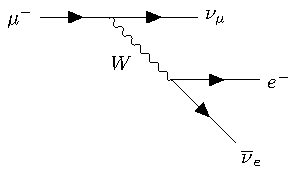
\includegraphics{Images/feynmanmuondecay.pdf}}
% \marginnote{
% \begin{center}
% \begin{tikzpicture}
%   \begin{feynman}
%     \vertex (i1) {$\mu^-$};
%     \vertex [right=of i1] (v1);
%     \vertex [below right=of v1] (v2);
%     \vertex [right=of v1] (f1) {$\nu_\mu$};
%     \vertex [right=of v2] (f2) {$e^-$};
%     \vertex [below right=of v2] (f3) {$\overline{\nu}_e$};
%     \diagram* {
%     (v1) -- [photon, edge label'=$W$] (v2),
%     (i1) -- [fermion] (v1),
%     (v1) -- [fermion] (f1),
%     (v2) -- [fermion] (f2),
%     (v2) -- [fermion] (f3),
%     };
%     \end{feynman}
% \end{tikzpicture}
% \end{center}}
and what we want to compute is:
\[
\pazocal{M}\{\mu^-(p_\mu,a)\xrightarrow[]{}e^-(p_e,b)+\overline{\nu}_e(\underset{\mathclap{\tikz \node {$\uparrow$} node [below=1ex] {\footnotesize $p_1$};}}{p_{\overline{\nu}_e}},c)+\nu_\mu(\underset{\mathclap{\tikz \node {$\uparrow$} node [below=1ex] {\footnotesize $p_2$};}}{p_{\nu_\mu}},d)\}
\]
The gauge bosons are massive, so we need to fix the gauge: in the unitary gauge, the propagator is given by: 
\[
-i\frac{g^{\alpha\beta}-k^\alpha k^\beta/m_W^2}{k^2-m^2_W+i\varepsilon}
\]
with $k^\alpha=(p_\mu)^\alpha-(p_2)^\alpha$. We need an additional \href{https://en.wikipedia.org/wiki/Richard_Feynman}{Feynman}
rule for this diagram: for each vertex in which there is an interaction with the $W$ boson, we obtain a factor $i\frac{g}{\sqrt{2}}\gamma^\alpha P_L$. With this said, and using the Feynman rules we already know, we get:
\[
\pazocal{M}=\overline{u}_b(p_e)\frac{ig}{\sqrt{2}}\gamma^\beta P_Lv_c(p_1)\frac{(-i)(g^{\alpha\beta}-k^\alpha k^\beta/m_W^2)}{k^2-m^2_W+i\varepsilon}\overline{u}_d(p_2)\frac{ig}{\sqrt{2}}\gamma_\alpha P_Lu_a(p_\mu)
\]
At this point, it is time to use some approximations:
\[
k^2\simeq p^2_\mu-2p_\mu\cdot p_2\sim\pazocal{O}(m_\mu^2) \quad m_\mu\sim0.1\text{ GeV} \quad m_W\sim10^2\text{ GeV}
\]
Hence, it follows:
\[
\frac{i}{m^2_W}\left(\frac{ig}{\sqrt{2}}\right)^2=-\frac{i}{2}\underbrace{\left(\frac{g^2}{m_W^2}{\color{red}\frac{\sqrt{2}}{8}}\right)}_{G_{\text{F}}}{\color{red}\frac{8}{\sqrt{2}}}=-\frac{4iG_{\text{F}}}{\sqrt{2}}
\]
With these approximations, we get:
\[
\pazocal{M}=\overline{u}_b(p_e)\gamma^\beta\left(\frac{1-\gamma^5}{2}\right)v_c(p_1)\overline{u}_d(p_2)\gamma^\beta\left(\frac{1-\gamma^5}{2}\right)u_a(p_\mu)\left(-\frac{4iG_{\text{F}}}{\sqrt{2}}\right)
\]
What we are really interested in is $\frac{1}{2}\sum_{a,b,c,d}\pazocal{M}(a,b,c,d)\pazocal{M}^*(a,b,c,d)$, which can be expressed as:
\[
\frac{1}{2}\sum_{a,b,c,d}\pazocal{M}(a,b,c,d)\pazocal{M}^*(a,b,c,d)=\left(\frac{G_{\text{F}}}{\sqrt{2}}\right)^2L_e^{\beta\gamma}(L_\mu)_{\beta\gamma}
\]
We focus for the moment on $L_e^{\beta\gamma}$:
\begin{align*}
L_e^{\beta\gamma}&=\overline{u}_b(p_e)\gamma^\beta(1-\gamma^5)v_c(p_1)v_c^\dagger(p_1)(1-\gamma^5)^\dagger(\gamma^\gamma)^\dagger\overline{u}_b^\dagger(p_e)\\
&=\overline{u}_b(p_e)\gamma^\beta(1-\gamma^5)v_c(p_1)\overline{v}_c(p_1)\gamma^0(1-\gamma^5)\gamma^0\gamma^\gamma\gamma^0\gamma^0u_b(p_e)\\
&=\overline{u}_b(p_e)\gamma^\beta(1-\gamma^5)v_c(p_1)\overline{v}_c(p_1)(1+\gamma^5)\gamma^\gamma u_b(p_e)
\end{align*}
Now, keep in mind that $\sum u(p)\overline{u}(p)=\slashed{p}+m$ and $\sum v(p)\overline{v}(p)=\slashed{p}-m$. For our purpose, in this part we can set $m_e=m_{\overline{\nu}_e}=m_{\nu_\mu}=0$ and finally we get:
\begin{align*}
L_e^{\beta\gamma}&=4\Tr{\gamma^\beta\left(\frac{1-\gamma^5}{2}\right)\slashed{p_1}\left(\frac{1+\gamma^5}{2}\right)\gamma^\gamma\slashed{p_e}}\\
&=4\Tr{\gamma^\beta\left(\frac{1-\gamma^5}{2}\right)\slashed{p_1}\gamma^\gamma\slashed{p_e}}\marginnote{We used the fact that $P_L^2=P_L$}
\end{align*}
To calculate the trace of this object, we use the following rules:
\[
\left\{
\begin{aligned}
&\Tr{\gamma^\mu\gamma^\nu\gamma^\rho\gamma^\sigma}=4\left(g^{\mu\nu}g^{\rho\sigma}-g^{\mu\rho}g^{\nu\sigma}+g^{\mu\sigma}g^{\nu\rho}\right)\\
&\Tr{\gamma^\mu\gamma^\nu\gamma^\rho\gamma^\sigma\gamma^5}=-4i\varepsilon^{\mu\nu\rho\sigma}; \quad \varepsilon^{\alpha\beta\mu\nu}\varepsilon_{\alpha\beta\rho\sigma}=-2(\delta^\mu_\rho\delta^\nu_\sigma-\delta^\mu_\sigma\delta^\nu_\rho)
\end{aligned}
\right.
\]
After repeating everything for $(L_\mu)_{\beta\gamma}$ and tedious calculations, we obtain:
\[
\frac{1}{2}\sum|\pazocal{M}|^2=64G^2_{\text{F}}(p_e\cdot p_2)(p_\mu\cdot p_1)
\]
We can compute the decay width, which is equal to:
\[
\Gamma=\frac{(2\pi)^4}{2m_\mu}\int\frac{d^3p_e}{(2\pi)^32E_e}\frac{d^3p_1}{(2\pi)^32E_1}\frac{d^3p_2}{(2\pi)^32E_2}\delta^4(p_\mu-p_e-p_1-p_2)\Braket{|\pazocal{M}|^2}
\]
Now, we integrate on $d^3p_e$:
\begin{align*}
\int\frac{d^3p_e}{2E_e}&=\int d^4p_e\theta(E_e)\delta(p_e^2-m_e^2)\delta^4(p_\mu-p_e-p_1-p_2)\\
&=\theta(E_\mu-E_1-E_2)\delta((p_\mu-p_1-p_2)^2)
\end{align*}
Suppose that we fix the direction of $p_1$ as the x-axis of our system: there is no dependence on the azimuth angle because the 3-body decay is planar, so $\int d\Omega_1=4\pi$ and $\int d\phi_{12}=2\pi$. We are in a reference system such that $p_\mu=(m_\mu,\Vec{0})$.
\begin{align*}
\Gamma=&\frac{64G_{\text{F}}^2}{8\pi^3m_\mu}\int_0^{+\infty}\frac{dE_1E_1^2}{2E_1}\frac{dE_2E_2^2}{2E_2}\int_{-1}^{+1}d\cos\theta_{12}\delta(\cdots)(p_e\cdot p_2)(p_\mu\cdot p_1)
\end{align*}
where the argument of the $\delta$ function is:
\[
m_\mu^2-2m_\mu(E_1+E_2)+2E_1E_2(1-\cos\theta_{12})
\]
When integrating it in $d\cos\theta_{12}$, keep in mind that it is possible to rewrite it as:
\[
\delta\left(\cos\theta_{12}-\frac{m_\mu^2-2m_\mu(E_1+E_2)+2E_1E_2}{2E_1E_2}\right)
\]
Hence, we have to see for which values of $E_1$ and $E_2$, $\cos\theta_{12}$ is in the interval [-1,+1]:
\[
\left\{
\begin{aligned}
E_1&: 0\le E_1\le m_\mu/2\\
E_2&: -1\le\frac{m_\mu^2-2m_\mu(E_1+E_2)+2E_1E_2}{2E_1E_2}\le1\Rightarrow\frac{m_\mu}{2}-E_1\le E_2\le\frac{m_\mu}{2}
\end{aligned}
\right.
\]
The upper limit on $E_1$ corresponds to having $e$ and $\nu_\mu (2)$ emitted in one direction and $\overline{\nu}_e (1)$ emitted in the other one, hence splitting the muon energy $m_\mu$ equally in the two directions. For $E_2$, we fix $E_1$ and do tedious calculations. The final result is:
\begin{align*}
\Gamma&=\frac{1}{2^5m_\mu\pi^3}\int_0^{m_\mu/2}dE_1E_1\int_{m_\mu/2-E_1}^{m_\mu/2}dE_2E_22^6G_{\text{F}}^2(p_e\cdot p_2)(p_\mu\cdot p_1)\\
&=\frac{G_{\text{F}}^2m_\mu^5}{192\pi^3}=\Gamma_0
\end{align*}
If we include the effects of electrons, we get some corrections:
\[
\Gamma=\Gamma_0(1-8r+8r^3-r^4-12r^4\ln r) \quad r=\left(\frac{m_e}{m_\mu}\right)^2
\]
We can estimate this decay width by taking into account that\\
$G_{\text{F}}\sim1/300^4$ GeV$^{-4}$ and $m_\mu^5\sim10^{-5}$ GeV$^5$. It follows
\[
\Gamma\sim10^{-19}\text{ GeV}\Rightarrow\tau_\mu=2.1\cdot10^{-6}\text{ s}
\]
\section{How to build a model/Lagrangian/EFT?}
\begin{figure}[h!]
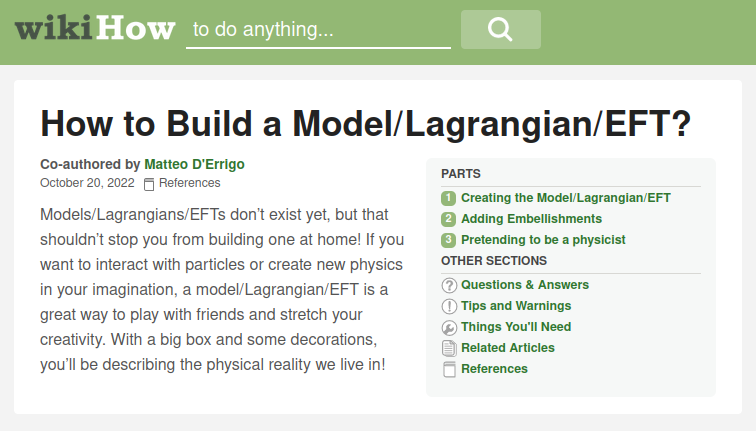
\includegraphics{Images/WikiHow.png}
\caption{WikiHow is not a good place to learn how to build a Lagrangian.}
\end{figure}
Our goal is to find the effective Lagrangian of nature, effective field theories (EFT) are characterized by certain degrees of freedom at a certain energy scale. To build a Lagrangian we have to:\marginnote{\textit{“Everything not forbidden is compulsory. — Marco Nardecchia”} — Michael Scott}
\begin{enumerate}
    \item specify the \textbf{local symmetries}, i.e. the gauge group G of the theory+Lorentz
    \item specify the \textbf{fields content}
    \item write the \textbf{most general Lagrangian} according to 1. and 2.
    \item spend several hours admiring the beautiful Lagrangian we just wrote and try to understand it without summoning any ancient demon
\end{enumerate}
Let's have a look at the case of QED:
\begin{table}[h]
    \centering
    \begin{tabular}{c|c|c}
        Field & G=U$(1)_{\text{C}}$ & Lorentz\\
        \hline
        $A_\mu$ & 0 & vector\\
        $\Psi_L$ & -1 & (1/2,0)\\
        $\Psi_R$ & -1 & (0,1/2)\\
        \hline
    \end{tabular}
    \caption*{}
    \labtab{qed}
\end{table}\\
The most general Lagrangian up to dimension 4 is given by:
\[
\pazocal{L}=-\frac{1}{4}F^{\mu\nu}F_{\mu\nu}+i\overline{\Psi}\gamma^\mu D_\mu\Psi-m\overline{\Psi}\Psi+\text{h.c.}
\]
with $F_{\mu\nu}=\partial_\mu A_\nu-\partial_\nu A_\mu$ and $D_\mu=i\partial_\mu-ieA_\mu$. Focus now on the Lagrangian without the mass term:
\[
\pazocal{L}=-\frac{1}{4}F^{\mu\nu}F_{\mu\nu}+i\overline{\Psi}_L\gamma^\mu D_\mu\Psi_L+i\overline{\Psi}_R\gamma^\mu D_\mu\Psi_R{\color{red}
-(m\overline{\Psi}_L\Psi_R+m^*\overline{\Psi}_R\Psi_L)}
\]
We can set $m=\hat{m}e^{i\theta}$ and $\Psi_L\xrightarrow[]{}\Psi'_L=\Psi_Le^{i\theta}$. In this way:
\[
(m\overline{\Psi}_L\Psi_R+m^*\overline{\Psi}_R\Psi_L)\xrightarrow[]{}(\hat{m}\overline{\Psi}'_L\Psi_R+\hat{m}\overline{\Psi}_R\Psi'_L)=m\overline{\Psi}\Psi
\]
In the case of QED, the group G=U$(1)_{\text{C}}=$U$(1)_{\text{L}}\times$U$(1)_{\text{R}}$ (2 generators) is broken into H=U$(1)_{\text{V}}$ (1 generator), i.e. $\Psi_{L/R}\xrightarrow[]{}e^{i\alpha}\Psi_{L/R}$:
\[
\left\{
\begin{aligned}
&\text{\# naive generators}=1 \text{ complex}=2 \text{ real}=\text{ modulus+phase}\\
&\text{\# broken generators}=2-1=1\\
&\text{\# physical parameters=\# naive-\# broken=1}
\end{aligned}
\right.
\]
\subsection{Review of the Standard Model}
For what concerns the Standard Model (SM), we have the gauge group given by G=SU$(3)_{\text{C}}\times$SU$(2)_{\text{L}}\times$U$(1)_{\text{Y}}$ and the fields content summarized in the table below:
    \begin{table}[h]
        \centering
        \begin{tabular}{c|c|c|c|c}
        \hline
        \rowcolor{gray!45}Field & SU$(3)_{\text{C}}$ & SU$(2)_{\text{EW}}$ & U$(1)_{\text{Y}}$ & SO(3,1) \\
        \hline
        \cellcolor{orange!45}$Q_L^i=\begin{pmatrix}
             u_L^i\\
             d_L^i 
        \end{pmatrix}$ & \cellcolor{orange!45}$\Box$ & \cellcolor{orange!45}$\Box$ & \cellcolor{orange!45}$+\frac{1}{6}$ &\cellcolor{orange!45} (2,1) \\
        \rowcolor{orange!45}$u_R^i$ & $\Box$ & 1 & $+\frac{2}{3}$ & (1,2) \\
        \rowcolor{orange!45}$d_R^i$ & $\Box$ & 1 & $-\frac{1}{3}$ & (1,2) \\
        \hline
        \cellcolor{orange!45}$L_L^i=\begin{pmatrix}\nu_L^i\\e_L^i\end{pmatrix}$ &\cellcolor{orange!45} 1 &\cellcolor{orange!45} $\Box$ &\cellcolor{orange!45} $-\frac{1}{2}$ &\cellcolor{orange!45} (2,1) \\
        \rowcolor{orange!45}$e_R^i$ & 1 & 1 & -1 & (1,2) \\
        \hline
        \rowcolor{blue!35}$G_\mu^{a=1,\dots,8}$ & Adj & 1 & 0 & (2,2)\\
        \rowcolor{blue!35}$W_\mu^{i=1,2,3}$ & 1 & Adj & 0 & (2,2)\\
        \rowcolor{blue!35}$B_\mu$ & 1 & 1 & 0 & (2,2)\\
        \hline
        \rowcolor{purple!45}$H$ & 1 & $\Box$ & $+\frac{1}{2}$ & (1,1)\\
        \hline
        \end{tabular}
        \caption{Field content in the Standard Model.}
        \labtab{SMfield}
    \end{table}\\
The Lagrangian is $\pazocal{L}=\pazocal{L}_{\text{kin}}+\pazocal{L}_{\text{Yuk}}+\pazocal{L}_\theta-V(H)$ plus some higher dimension operators. The four different pieces are:
    \[
    \left\{
    \begin{aligned}
    &\pazocal{L}_{\text{kin}}=-\frac{1}{4}(G_{\mu\nu}^a)^2-\frac{1}{4}(W_{\mu\nu}^i)^2-\frac{1}{4}(B_{\mu\nu})^2+|D_\mu H|^2+\sum_{\{\Psi\}}\sum_{j=1}^{3}\overline{\Psi}_ji\slashed{D}\Psi_j\\
    &\pazocal{L}_\theta=\frac{\theta_0}{32\pi^2}G_{\mu\nu}^a\Tilde{G}^{\mu\nu,a}\\
    &\pazocal{L}_{\text{Yuk}}=-\sum_{i,j=1}^3\left[\overline{Q}_L^i(Y_u)^{ij}H^cu_R^j+\overline{Q}_L^i(Y_d)^{ij}Hd_r^j+\overline{L}_L^i(Y_l)^{ij}He_R^j+\text{h.c}\right]\\
    &V(H)=-\mu^2H^\dagger H+\lambda(H^\dagger H)^2
    \end{aligned}
    \right.
    \]
$Y_u$, $Y_d$ and $Y_l$ are $3\times3$ matrices in flavour space. We know that $\Box$ of SU(2) is a pseudo-real representation, $H$ is the $\Box$ of SU(2) so it is always possible to form another $\Box$ of SU(2): $H^c:=i\sigma^2H^*$. It transforms as a doublet, we use it to build the Yukawa coupling and we use $H^c$ because it has hypercharge -1/2.\\
The \textbf{fermions} (matter fields), highlighted in orange in the table, are formed by quarks and leptons. Quarks come in triplet of colours, left-handed quarks and leptons come in doublets of weak isospin, where $i$ is the family index $i=1,2,3$. The fact that left- and right-handed fermions carry different weak isospin makes the Standard Model a chiral gauge theory. There is no right-handed neutrino because we do not need it now, we want the minimum number of fields which reproduce what is observed in nature, although there is evidence for neutrino masses from neutrino oscillations experiments. The threefold replication of quark-lepton families is one of the
puzzles whose explanation requires physics beyond the Standard Model.\\
The spin-1 particles are the \textbf{gauge bosons} associated with the fundamental interactions, highlighted in blue in the table: $G_\mu^a$ are the \textbf{gluons} of the \textbf{strong interaction}, $W_\mu^i$ and $B_\mu$ are the bosons of the \textbf{electroweak interaction}.\\
The last ingredient of the Standard Model is the \textbf{Higgs field}, the only spin-0 particle in the theory, highlighted in purple in the table. It is a complex scalar field and a doublet of weak isospin, coupling left- and right-handed fermions together.

We now look at the potential $V(H)$. It must be invariant under SU(2), so there cannot be cubic terms.  First of all, we have to choose the right parametrization for the Higgs field $H$: there are 4 degrees of freedom, so we can put three of them on an exponential and the last one as a multiplicative constant.
\[
H(x)=e^{i\overset{\mathclap{\tikz \node {$\downarrow$} node [above=1ex] {\footnotesize  Nambu-Goldstone bosons};}}{\chi^i(x)}\sigma^i}\left(\begin{array}{c}0\\\frac{\phi(x)}{\sqrt{2}}\end{array}\right)
\]
Substituting this form of $H$ into the expression for the potential $V(H)$, we find out that this is only a function of $\phi(x)$:
\[
V(H)\xrightarrow[]{}V(\phi)=-\frac{1}{2}\mu^2\phi^2+\frac{1}{4}\lambda\phi^4
\]
This potential has two minima in $\pm v$, where $v=\sqrt{\frac{\mu^2}{\lambda}}=\langle\phi\rangle$: the field $\phi(x)$ can be written as its vacuum expectation value plus an excitation which turns out to be the Higgs boson:
\[
\phi(x)=\frac{v+h(x)}{\sqrt{2}}
\]
$h(x)$ is the radial excitation while $\chi(x)$ is the angular excitation: the latter costs no energy since $V(\phi)$ does not depend on $\chi$, therefore the NGBs are massless. We have the SSB mechanism here: how do we understand which symmetry we are breaking? We write the vev and see what symmetry is left invariant.\marginnote{From \cite{schwartz}, Section 29.1.}
\[
\Braket{H(x)}=\frac{1}{\sqrt{2}}\begin{pmatrix}
    0\\v
\end{pmatrix}
\]
Now we act with a combination of generators from SU(2)$\times$U(1), which is $a_i\frac{\sigma_i}{2}+a_0Y$. We want to see when $(a_i\frac{\sigma_i}{2}+a_0Y)\langle H(x)\rangle=0$.
\begin{align*}
\left(a_i\frac{\sigma_i}{2}+a_0Y\right)\langle H(x)\rangle&=\frac{1}{2}\left(\begin{array}{cc}
    2a_0+a_3 & a_1-ia_2 \\
    a_1+ia_2 & 2a_0-a_3
\end{array}\right)\begin{pmatrix}
    0\\1
\end{pmatrix}\\
&=\frac{1}{2}\begin{pmatrix}
    a_1-ia_2\\2a_0-a_3
\end{pmatrix}
\begin{pmatrix}
    0\\1
\end{pmatrix}=\begin{pmatrix}
    0\\0
\end{pmatrix}\Rightarrow\left\{\begin{aligned}
    &a_1=a_2=0\\
    &a_0=\frac{1}{2}a_3
\end{aligned}\right.
\end{align*}
The \textbf{unbroken generator} is $Q=T_3+\frac{1}{2}Y$, the Higgs scalar potential breaks SU$(2)_{\text{EW}}\times$U$(1)_{\text{Y}}$ into U$(1)_{\text{Q}}$, i.e. 3+1 generators are broken into 1, resulting in 3 massless modes.\\
We now want to see masses and couplings, so we move in the unitary gauge where $\chi^i=0$. In the unitary gauge the potential will depend on $h(x)$, resulting in:
\[
V(H)=\frac{1}{2}m_h^2h^2(x)+\lambda vh^3(x)+\frac{1}{4}\lambda h^4(x)+\text{constant terms}
\]
with $m_h^2=2\mu^2=2v^2\lambda$. We need the masses for the vector bosons, so we look at the kinetic term
$|D_\mu H|^2=(D_\mu H)^\dagger(D_\mu H)$. Here the covariant derivative is defined as:
\[
D_\mu H=\frac{1}{\sqrt{2}}\left[\partial_\mu-\frac{i}{2}(gW_\mu^i\sigma^i+g'Y_WB_\mu)\right]\begin{pmatrix}0 \\ v+h(x)\end{pmatrix}
\]
where $g$ is the gauge coupling of SU(2) and $g'$ the gauge coupling of U(1)$_{\text{Y}}$.\\
Before proceeding with the calculations, we define $W_\mu^\pm$ as a linear combination of $W_\mu^1$ and $W_\mu^2$: 
\[
W_\mu^\pm:=\frac{1}{\sqrt{2}}(W_\mu^1\mp iW_\mu^2)
\]
and the same can be done for the $\sigma$ matrices, i.e. $\sigma^\pm:=\frac{1}{2}(\sigma^1\pm i\sigma^2)$, so that it is possible to write:
\begin{align*}
W_\mu^+\sigma^++W_\mu^-\sigma^-=&\frac{1}{2\sqrt{2}}(W_\mu^1-iW_\mu^2)(\sigma^1+i\sigma^2)\\
&+\frac{1}{2\sqrt{2}}(W_\mu^1+iW_\mu^2)(\sigma^1-i\sigma^2)\\
=&\frac{1}{2\sqrt{2}}(W_\mu^1\sigma^1+\cancel{iW_\mu^1\sigma^2}-\cancel{iW_\mu^2\sigma^1}+W_\mu^2\sigma^2)\\
&+\frac{1}{2\sqrt{2}}(W_\mu^1\sigma^1-\cancel{iW_\mu^2\sigma^2}+\cancel{iW_\mu^2\sigma^1}+W_\mu^2\sigma^2)\\
=&\frac{1}{\sqrt{2}}(W_\mu^1\sigma^1+W_\mu^2\sigma^2)
\end{align*}
From which it follows that:
\[
W_\mu^1\sigma^1+W_\mu^2\sigma^2+W_\mu^3\sigma^3=\sqrt{2}(W_\mu^+\sigma^++W_\mu^-\sigma^-)+W_\mu^3\sigma^3
\]
$D_\mu H$ now becomes:
\begin{align*}
D_\mu H=&\frac{1}{\sqrt{2}}\begin{pmatrix}0 \\ \partial_\mu h(x)\end{pmatrix}-\frac{i}{2\sqrt{2}}(gW_\mu^3\sigma^3+g'Y_WB_\mu)\begin{pmatrix}0 \\ v+h(x)\end{pmatrix}\\
&-\frac{ig}{2}(W_\mu^+\sigma^++W_\mu^-\sigma^-)\begin{pmatrix}0 \\ v+h(x)\end{pmatrix}
\end{align*}
When we act with $\sigma^3$, $\sigma^+$ and $\sigma^-$ on $H(x)$ we get:
\[
\left\{
\begin{aligned}
&\sigma^3H(x)=\left(\begin{array}{cc}
    1 & 0 \\
    0 & -1
\end{array}\right)\left(\begin{array}{c}
  0 \\
  v+h(x)
\end{array}\right)=-\left(\begin{array}{c}
  0 \\
  v+h(x)
\end{array}\right) \\
&\sigma^+H(x)=\left(\begin{array}{cc}
    0 & 1 \\
    0 & 0
\end{array}\right)\left(\begin{array}{c}
  0 \\
  v+h(x)
\end{array}\right)=+\left(\begin{array}{c}
  v+h(x) \\
  0
\end{array}\right) \\
&\sigma^-H(x)=\left(\begin{array}{cc}
    0 & 0 \\
    1 & 0
\end{array}\right)\left(\begin{array}{c}
  0 \\
  v+h(x)
\end{array}\right)=\left(\begin{array}{c}
  0 \\
  0
\end{array}\right)
\end{aligned}
\right.
\]
Substituting this into the previous expression for $D_\mu H$, one finds:
\begin{align*}
D_\mu H=&\frac{1}{\sqrt{2}}\begin{pmatrix}0 \\ \partial_\mu h(x)\end{pmatrix}+\frac{i}{2\sqrt{2}}(gW_\mu^3-g'Y_WB_\mu)\begin{pmatrix}0 \\ v+h(x)\end{pmatrix}\\
&-\frac{ig}{2}W_\mu^+\begin{pmatrix}v+h(x) \\ 0 \end{pmatrix}
\end{align*}
With the same strategy, we compute $(D_\mu H)^\dagger$:
\begin{align*}
(D_\mu H)^\dagger=&\begin{pmatrix}0 & v+h(x)\end{pmatrix}\frac{1}{\sqrt{2}}\left[\partial_\mu+\frac{i}{2}(g\sigma^iW_\mu^i+g'Y_WB_\mu)\right]\\
=&\frac{1}{\sqrt{2}}\begin{pmatrix}0 & \partial_\mu h(x)\end{pmatrix}\\
&+\frac{i}{2\sqrt{2}}\begin{pmatrix}0 & v+h(x)\end{pmatrix}(g\sigma^3W_\mu^3+g'Y_WB_\mu)\\
&+\frac{ig}{2}\begin{pmatrix}0 & v+h(x)\end{pmatrix}(\sigma^+W_\mu^++\sigma^-W_\mu^-)\marginnote{We act with the $\sigma$ matrices on the row vector: $\sigma^3$ changes its sign as before, $\sigma^+$ gives a zero while $\sigma^-$ flips it.}\\
=&\frac{1}{\sqrt{2}}\begin{pmatrix}0 & \partial_\mu h(x)\end{pmatrix}-\frac{i}{2\sqrt{2}}\begin{pmatrix}0 & v+h(x)\end{pmatrix}(gW_\mu^3-g'Y_WB_\mu)\\
&+\frac{ig}{2}\begin{pmatrix}v+h(x) & 0\end{pmatrix}W_\mu^-
\end{align*}
We can finally write the full form of $|D_\mu H|^2$:
\begin{align*}
|D_\mu H|^2=&(D_\mu H)^\dagger(D_\mu H)\\
=&\frac{1}{2}(\partial_\mu h(x))^2+\frac{(v+h(x))^2}{8}(gW_\mu^3-g'B_\mu)^2\\
&+\frac{g^2}{4}(v+h(x))^2W_\mu^+W_\mu^-\\
=&\frac{1}{2}(\partial_\mu h(x))^2+\frac{v^2}{8}(gW_\mu^3-g'B_\mu)^2\left(1+\frac{h(x)}{v}\right)^2\\
&+\frac{g^2v^2}{4}W_\mu^+W_\mu^-\left(1+\frac{h(x)}{v}\right)^2
\end{align*}
At this point, we can identify the mass of the $W$ boson as:
\begin{kaobox}[frametitle=Mass of the $W$ boson]
\[
m_W:=\frac{1}{2}gv
\]    
\end{kaobox}
To explicitly see the mass of the $Z$ boson $m_Z$ we perform a rotation. Let $A_\mu$ be the massless field and $Z_\mu$ the massive one:
\[
\left(\begin{array}{c}
     A_\mu \\
     Z_\mu
\end{array}\right)=\left(\begin{array}{cc}
    \cos\theta_w & \sin\theta_w \\
    -\sin\theta_w & \cos\theta_w
\end{array}\right)\left(\begin{array}{c}
     B_\mu \\
     W_\mu^3 
\end{array}\right)
\]
From this rotation, it follows that:
\begin{equation}
\labeq{azbasis}
\left\{
\begin{aligned}
&A_\mu=\sin\theta_wW_\mu^3+\cos\theta_wB_\mu\\
&Z_\mu=\cos\theta_wW_\mu^3-\sin\theta_wB_\mu
\end{aligned}
\right.
\Leftrightarrow
\left\{
\begin{aligned}
&B_\mu=\cos\theta_wA_\mu-\sin\theta_wZ_\mu\\
&W_\mu^3=\sin\theta_wA_\mu+\cos\theta_wZ_\mu
\end{aligned}
\right.
\end{equation}
$\theta_w$ is the \href{https://en.wikipedia.org/wiki/Steven_Weinberg}{Weinberg} angle. To write the mass term $m_Z^2$ in the expression of $|D_\mu H|^2$, we have to perform some tricks:
\[
{\color{red}\frac{g^2+g'^2}{g^2+g'^2}}\frac{v^2}{8}(gW_\mu^3-g'B_\mu)^2=\frac{m_Z^2}{2}\left(\frac{g}{\sqrt{g^2+g'^2}}W_\mu^3-\frac{g'}{\sqrt{g^2+g'^2}}B_\mu\right)^2
\]
To obtain the desired result, we express $\theta_w$ in terms of the couplings $g$ and $g'$:
\begin{equation}
\labeq{thetaw}  
\sin\theta_w:=\frac{g'}{\sqrt{g^2+g'^2}} \quad \cos\theta_w:=\frac{g}{\sqrt{g^2+g'^2}} \quad \tan\theta_w=\frac{g'}{g}
\end{equation}
In this way, it is possible to define:
\begin{kaobox}[frametitle=Mass of the $Z$ boson]
\[
m_Z:=\frac{1}{2}v\sqrt{g^2+g'^2}=\frac{1}{2}\frac{gv}{\cos\theta_w}=\frac{m_W}{\cos\theta_w}\marginnote{The subscript with capital W is for the $W$ boson, while the one with small w is for the Weinberg angle.}
\]    
\end{kaobox}
$|D_\mu H|^2$ now can be written as:
\[
|D_\mu H|^2=\frac{1}{2}(\partial_\mu h)^2+\frac{1}{2}m_Z^2Z_\mu Z^\mu\left(1+\frac{h}{v}\right)^2+m_W^2W_\mu^+W_\mu^-\left(1+\frac{h}{v}\right)^2
\]
We have the three fields that will acquire mass, the only remaining massless field is the photon. The mass terms cannot be included in the Lagrangian, since terms of the form $m\overline{\Psi}\Psi$ do not respect U$(1)\times$SU$(2)_L$ gauge invariance.\\
The Standard Model has 18 physical parameters, it does not matter how we write them, we could parameterize the SM in different ways but the number of physical parameters does not change. To see how to count these parameters, let's take a look at the leptonic Yukawa term:
\[
\overline{l}_L^i(Y_e)^{ij}He_R^j
\]
$Y_e$ is a 3$\times$3 complex matrix, so it contains 18 real parameters. However, the SM lepton sector only has 3 physical parameters (the masses of the charged leptons): there are 15 hidden unphysical parameters. Since they are useless for predictions, it is better to choose a parametrization where everything is physical.\\
Where do the 18 physical parameters come from?\marginnote{\href{https://www.youtube.com/watch?v=_IXfPxe7j6o&themeRefresh=1}{Phenomenological explanation} of the 18 parameters.} We have the \textbf{three coupling constants} $g, g'$ and $g_s$ which determine the strength of each force, from the Higgs sector we have the \textbf{vacuum expectation value} $v$ and the \textbf{interaction strength} $\lambda$, while from the Yukawa sector we get the \textbf{three charged lepton masses} plus \textbf{ten physical parameters} associated with the quark Yukawa sector. 
\section{Symmetries}
\subsection{Parity}
We already know that we can parameterize our field as composed by a left-handed spinor $\xi$ and a right-handed spinor $\eta$:
\[
\Psi=\left(\begin{array}{c}
     \xi\\
     \eta
\end{array}\right)
\quad
\left\{
\begin{aligned}
&\xi=(2,1) \text{ of Lorentz}\\
&\eta=(1,2) \text{ of Lorentz}
\end{aligned}
\right.
\]
Moreover, we have that under parity position and momentum transform as:
\[
(\Vec{x},t)\xrightarrow[]{}(-\Vec{x},t) \quad \Vec{p}\xrightarrow[]{}-\Vec{p}
\]
while the spin remains untouched being a pseudo-vector. This means that the \textbf{helicity} gets flipped under parity transformations. For the right- and left-handed spinors, we have the relation $\xi(\Vec{x,t})\xleftrightarrow[]{}\eta(-\Vec{x},t)$ and can introduce an intrinsic parity of the field, i.e. a phase:
\[
\left\{
\begin{aligned}
&\xi(\Vec{x},t)\xrightarrow[]{}\zeta_p\eta(-\Vec{x},t)\\
&\eta(\Vec{x},t)\xrightarrow[]{}\zeta_p\xi(-\Vec{x},t)
\end{aligned}
\right.
\]
In terms of $\Psi$ we have $\Psi(\Vec{x},t)\xrightarrow[]{}\zeta_p\gamma^0\Psi(-\Vec{x},t).$\marginnote{The gamma matrices are defined as:
\[
\gamma^\mu=\left(\begin{array}{cc}
    0 & \sigma^\mu \\
    \overline{\sigma}^\mu & 0
\end{array}\right), \gamma^5=\left(\begin{array}{cc}
    -1 & \\
     & -1
\end{array}\right)
\]
with $\sigma^\mu=(\mathbb{1},\sigma^i)$, $\overline{\sigma}^\mu=(\mathbb{1},-\sigma^i)=\eta_{\mu\mu}\sigma^\mu$ and $\eta_{\mu\mu}=(+1,-1,-1,-1)$} We can have a look at the current under parity:
\begin{align*}
\overline{\Psi}\gamma^\mu\Psi=\Psi^\dagger\gamma^0\gamma^\mu\Psi=\xi^\dagger\overline{\sigma}^\mu\xi+\eta^\dagger\sigma^\mu\eta\xrightarrow[\text{parity}]{}&\eta^\dagger\overline{\sigma}^\mu\eta+\xi^\dagger\sigma^\mu\xi\\
&=\eta_{\mu\mu}(\eta^\dagger\sigma^\mu\eta+\xi^\dagger\overline{\sigma}^\mu\xi)\\
&=\eta_{\mu\mu}\overline{\Psi}\gamma^\mu\Psi
\end{align*}
This is just a vector, now we include $A_\mu(\Vec{x},t)\xrightarrow[]{}\eta_{\mu\mu}A_\mu(-\Vec{x},t)$: it follows that $A_\mu\overline{\Psi}\gamma^\mu\Psi$ is invariant, hence QED is invariant under parity. The same results apply for QCD, since $G_\mu^a\overline{\Psi}\lambda^a\gamma^\mu\Psi$ is invariant. On the other hand, the theta term is odd under parity: it is proportional to $G_{\mu\nu}G_{\rho\sigma}\varepsilon^{\mu\nu\rho\sigma}$ and $\varepsilon$ forces 3 indices to be space-like and 1 to be time-like.
\subsection{Charge conjugation}
We now see what happens when we transform the field $\Psi$ under charge conjugation:
\[
\Psi(x)\xrightarrow[]{C}i\gamma_2\Psi^*(x)\Tilde{\eta}_\Psi
\quad
\left\{
\begin{aligned}
&\xi(x)\xrightarrow[]{C}\Tilde{\eta}_\Psi\eta^c(\Vec{x},t) \,\text{ with }\, \eta^c=i\sigma^2\eta^*\\
&\eta(x)\xrightarrow[]{C}-\Tilde{\eta}_\Psi\xi^c(\Vec{x},t) \,\text{ with }\, \xi^c=i\sigma^2\xi^*
\end{aligned}
\right.
\]
Moreover, we have that $\eta^\dagger\sigma^\mu\eta=-\eta^{c\dagger}\overline{\sigma}^\mu\eta^c$:
\begin{align*}
-\eta^{c\dagger}\overline{\sigma}^\mu\eta^c&=-(i\sigma^2\eta^*)^\dagger\overline{\sigma}^\mu(i\sigma^2\eta^*)=-\eta^T\underbrace{\sigma_2\overline{\sigma}^\mu\sigma_2}_{\sigma^{\mu T}}\eta^*\\
&=-\eta^T\sigma^{\mu T}\eta^*=\eta^\dagger\sigma^\mu\eta
\end{align*}
What happens now if we do $C^\dagger A_\mu(x)C$? We obtain just a phase $\eta_A$ since photons are real particles.

The QCD case is more complicated: we have $\overline{\Psi}_\alpha\gamma^\mu\frac{\lambda^a_{\alpha\beta}}{2}G_\mu^a\Psi_\beta$ and we ask ourselves how does $\overline{\Psi}_\alpha\gamma^\mu\Psi_\beta$ transform under charge conjugation.
\[
\left\{
\begin{aligned}
&\overline{\Psi}_\alpha\gamma^\mu\Psi_\beta\xrightarrow[]{C}-\overline{\Psi}_\beta\gamma^\mu\Psi_\alpha\Tilde{\eta}_{\Psi_\alpha}\Tilde{\eta}^*_{\Psi_\beta}\\
&\overline{\Psi}_\alpha\gamma^\mu\frac{\lambda^a_{\alpha\beta}}{2}\Psi_\beta\xrightarrow[]{C}\overline{\Psi}\gamma^\mu\frac{(\lambda^a)^T}{2}\Psi\\
&G_\mu^a\lambda^a\xrightarrow[]{C}-G_\mu^a(\lambda^a)^T\Rightarrow C^\dagger G_\mu^a C=\Tilde{\eta}_{G_\mu}G_\mu^a
\end{aligned}
\right.
\]
The phase $\Tilde{\eta}_{G_\mu}$ depends on the generators:
\[
\left\{
\begin{aligned}
&(\lambda^a)^T=\lambda^a &&\text{ for } \, a=1,3,4,6,8\Rightarrow\Tilde{\eta}_{G_\mu}=-1\\
&(\lambda^a)^T=-\lambda^a &&\text{ for } \, a=2,5,7\Rightarrow\Tilde{\eta}_{G_\mu}=+1
\end{aligned}
\right.
\]
\subsection{Discrete Symmetries}
We are now going to review discrete symmetries, focusing on states, creation/annihilation  operators and fields:\marginnote{$A$ is just an internal quantum number.}
\[
\ket{A,\Vec{p},\sigma}\xrightarrow[\text{parity}]{}\left\{
\begin{aligned}
&\hat{P}\ket{A,\Vec{p},\sigma}=\eta_A\ket{A,-\Vec{p},\sigma}\\
&\hat{P}\ket{\overline{A},\Vec{p},\sigma}=\eta_{\overline{A}}\ket{\overline{A},-\Vec{p},\sigma}
\end{aligned}
\right.
\]
The operators $\hat{a}^\dagger, \hat{a}$ refer to particles while $\hat{b}^\dagger, \hat{b}$ refer to anti-particles:
\[
\hat{P}\hat{a}^\dagger_\sigma(\Vec{p})\hat{P}^\dagger\ket{0}=\eta_A\hat{a}^\dagger_\sigma(-\Vec{p})\ket{0}\Rightarrow\left\{
\begin{aligned}
&\hat{P}\hat{a}^\dagger_\sigma(\Vec{p})\hat{P}^\dagger=\eta_A\hat{a}^\dagger_\sigma(-\Vec{p})\\
&\hat{P}\hat{b}^\dagger_\sigma(\Vec{p})\hat{P}^\dagger=\eta_{\overline{A}}\hat{b}^\dagger_\sigma(-\Vec{p})
\end{aligned}
\right.
\]
Now we want the transformation rules for the fields: $\hat{P}\phi(x)\hat{P}^\dagger=?$ For scalar fields, we have:
\[
\hat{P}\phi(x)\hat{P}^\dagger=\eta_\phi\phi(\pazocal{P}x) \, \text{ with } \, \pazocal{P}=\text{diag}(+1,-1,-1,-1)
\]
Furthermore, we know how to express the field $\phi(x)$ in terms of creation and annihilation operators:
\[
\phi(x)=\int \frac{d^3p}{(2\pi)^3}\frac{1}{\sqrt{2E_p}}\left[\hat{a}(\Vec{p})e^{-ipx}+\hat{b}^\dagger(\Vec{p})e^{+ipx}\right]
\]
Acting with parity on $\phi(x)$, in order to get the previous form, it has to be $\eta_\phi=\eta_A^*$ and $\eta_A\eta_{\overline{A}}=1$.\\
It is possible to repeat the same procedure for fermions:
\[
\Psi(x)=\sum_\sigma\int \frac{d^3p}{(2\pi)^3}\frac{1}{2E(\Vec{p})}\left[\hat{a}_\sigma(\Vec{p})e^{-ipx}u(\Vec{p})+\hat{b}^\dagger_\sigma(\Vec{p})e^{+ipx}v(\Vec{p})\right]
\]
We now act with the parity operator $\hat{P}$:
\begin{align*}
\hat{P}\Psi(x)\hat{P}^\dagger=\eta_\Psi\gamma^0\Psi(\pazocal{P}x)=\sum_\sigma\int \frac{d^3p}{(2\pi)^32E(\Vec{p})}&\left[\eta_A^*\hat{a}_\sigma(-\Vec{p})e^{-ipx}u(\Vec{p})\right.\\
&\left.+\eta_{\overline{A}}\hat{b}^\dagger_\sigma(-\Vec{p})e^{+ipx}v(\Vec{p})\right]
\end{align*}
The field $\Psi$ is now not calculated in $x$ but in $\pazocal{P}x$. For the spinors, this means $u(\Vec{p})=\gamma^0u(\pazocal{P}\Vec{p})$ and $v(\Vec{p})=-\gamma^0v(\pazocal{P}\Vec{p})$. What we get at the end is that $\eta_\Psi=\eta_A^*$ and $\eta_A\eta_{\overline{A}}=-1$.

Suppose now to have an Abelian symmetry, which translates into $U(\theta)\ket{A,\Vec{p},\sigma}=e^{iq_A\theta}\ket{A,\Vec{p},\sigma}$, and to apply parity to it:
\[
\hat{P}U(\theta)\ket{A,\Vec{p},\sigma}=\underbrace{e^{iq_A\theta}\eta_A}_{\eta'_A}\ket{A,-\Vec{p},\sigma}
\]
We can redefine $\eta'_A$ to be equal to 1. Doing this, we also define a new operator $\hat{P}'=\hat{P}U(\theta=-\arg(\eta_A)/q_A)$. This is possible only when there is a global symmetry associated.
\begin{table}[h]
    \centering
    \begin{tabular}{c|c|c|c}
    \rowcolor{gray!45}State & $\eta$ & Global symmetry & Theory\\
    \hline
    Lepton & +1 & U$(1)_e\times$U$(1)_\mu\times$U$(1)_\tau$ & QED\\
    Anti-lepton & -1 & U$(1)_e\times$U$(1)_\mu\times$U$(1)_\tau$ & QED\\
    Quarks & +1 & U$(1)^{N_F}$ & QCD+QED\\
    Anti-quarks & -1 & U$(1)_u\times$U$(1)_d\times$U$(1)_s$ & QCD+QED\\
    \hline
    \end{tabular}
    \caption*{}
    \labtab{boh}
\end{table}
\end{document}